\documentclass[11pt, oneside]{article}
\usepackage{geometry}
\geometry{letterpaper}
\usepackage{graphicx}
\usepackage{amssymb}
\usepackage{amsmath}
\usepackage{tikz}
\usepackage{tikz-qtree}
\usepackage{url}
\usepackage[T1]{fontenc}

\title{SICP Exercise 3.12}
\author{Yuchong Pan}

\begin{document}
\maketitle

The missing \emph{<response>}s are \textbf{(b)} and \textbf{(b c d)}, respectively. The box-and-pointer diagrams are given as follows.

\begin{figure}[h!]
    \centering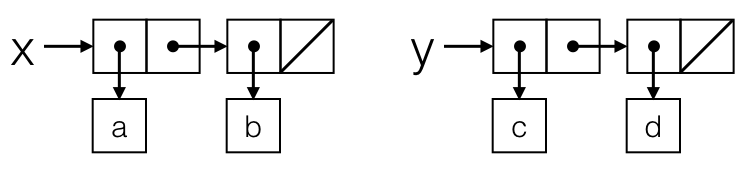
\includegraphics[width=10cm]{ex-3.12-1.png}
    \caption{Lists x: \textbf{(a b)} and y: \textbf{(c d)}.}
\end{figure}

\begin{figure}[h!]
    \centering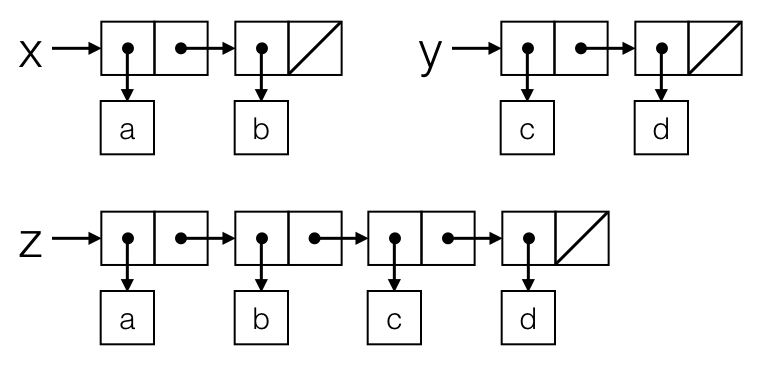
\includegraphics[width=10cm]{ex-3.12-2.png}
    \caption{Effect of \textbf{(define z (append x y))}.}
\end{figure}

\begin{figure}[h!]
    \centering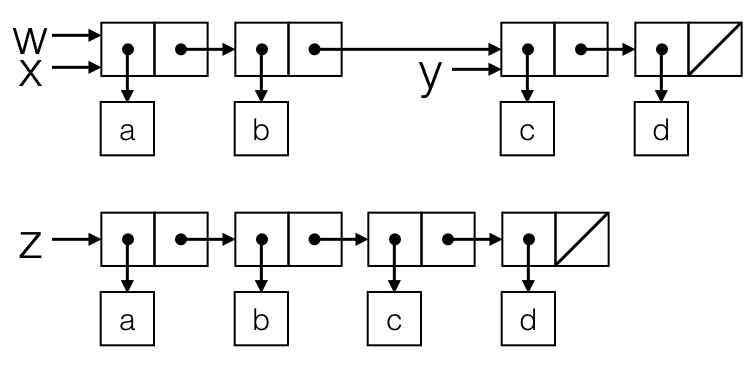
\includegraphics[width=10cm]{ex-3.12-3.png}
    \caption{Effect of \textbf{(define w (append! x y))}.}
\end{figure}

\end{document}
